\documentclass[convert, border=2pt,outext=.png]{standalone}

\usepackage[utf8]{inputenc}
\usepackage{lmodern}
\usepackage[T1]{fontenc}

\usepackage{bm}

\usepackage{tikz}
\usepackage[europeanvoltages, europeancurrents, europeanresistors]{circuitikz}
\usepackage{pgfplots}
\usetikzlibrary{positioning}
\usetikzlibrary{plotmarks}
\usetikzlibrary{backgrounds}
\usetikzlibrary{arrows,arrows.meta}
\usetikzlibrary{decorations,decorations.markings,decorations.pathreplacing,decorations.pathmorphing}
\usetikzlibrary{calc,math}
\usetikzlibrary{patterns,patterns.meta}
\usetikzlibrary{shapes,shapes.symbols,shapes.geometric}

\tikzstyle{block} = [draw, fill=white, rectangle, minimum height=3em, minimum width=4em]
\tikzstyle{rblock} = [draw, fill=white, circle, inner sep=0pt,minimum size=1mm]
\tikzstyle{wobblock} = [fill=white, rectangle, minimum height=3em, minimum width=5em]
\tikzstyle{nlblock} = [draw, postaction={draw,line width=0.25mm,white}, line width=0.5mm, black, fill=white, rectangle, minimum height=3em, minimum width=5em]
\tikzstyle{sum} = [draw,circle]
\tikzstyle{branch} = [circle,inner sep=0pt,minimum size=1mm,fill=black,draw=black]
\tikzstyle{nvbranch} = [circle,inner sep=0pt,minimum size=1mm,fill=white,draw=white, fill opacity=0, draw opacity=0]
\tikzstyle{vecBranch} = [circle,inner sep=0pt,minimum size=2mm,fill=black,draw=black]
\tikzstyle{input} = [coordinate]
\tikzstyle{output} = [coordinate]
\tikzstyle{coord} = [coordinate]
\tikzstyle{pinstyle} = [pin edge={<-,thin,black,>=latex'}]

\makeatletter
\pgfdeclaredecoration{coilup}{coil}
{
  \state{coil}[switch if less than=%
    1.5\pgfdecorationsegmentlength+%
    \pgfdecorationsegmentaspect\pgfdecorationsegmentamplitude+%
    \pgfdecorationsegmentaspect\pgfdecorationsegmentamplitude to last,
               width=+\pgfdecorationsegmentlength]
  {
    \pgfpathcurveto
    {\pgfpoint@oncoil{0    }{ 0.555}{1}}
    {\pgfpoint@oncoil{0.445}{ 1    }{2}}
    {\pgfpoint@oncoil{1    }{ 1    }{3}}
    \pgfpathmoveto{\pgfpoint@oncoil{1    }{-1    }{9}}
    \pgfpathcurveto
    {\pgfpoint@oncoil{0.445}{-1    }{10}}
    {\pgfpoint@oncoil{0    }{-0.555}{11}}
    {\pgfpoint@oncoil{0    }{ 0    }{12}}
  }
  \state{last}[width=.5\pgfdecorationsegmentlength+%
    \pgfdecorationsegmentaspect\pgfdecorationsegmentamplitude+%
    \pgfdecorationsegmentaspect\pgfdecorationsegmentamplitude,next state=final]
  {
    \pgfpathcurveto
    {\pgfpoint@oncoil{0    }{ 0.555}{1}}
    {\pgfpoint@oncoil{0.445}{ 1    }{2}}
    {\pgfpoint@oncoil{1    }{ 1    }{3}}
    \pgfpathmoveto{\pgfpoint@oncoil{2    }{ 0    }{6}}
  }
  \state{final}
  {
  \pgfpathmoveto{\pgfpointdecoratedpathlast}
  }
}

\pgfdeclaredecoration{coildown}{coil}
{
  \state{coil}[switch if less than=%
    1.5\pgfdecorationsegmentlength+%
    \pgfdecorationsegmentaspect\pgfdecorationsegmentamplitude+%
    \pgfdecorationsegmentaspect\pgfdecorationsegmentamplitude to last,
               width=+\pgfdecorationsegmentlength]
  {
    \pgfpathmoveto{\pgfpoint@oncoil{1    }{1    }{3}}
    \pgfpathcurveto
    {\pgfpoint@oncoil{1.555}{ 1    }{4}}
    {\pgfpoint@oncoil{2    }{ 0.555}{5}}
    {\pgfpoint@oncoil{2    }{ 0    }{6}}
    \pgfpathcurveto
    {\pgfpoint@oncoil{2    }{-0.555}{7}}
    {\pgfpoint@oncoil{1.555}{-1    }{8}}
    {\pgfpoint@oncoil{1    }{-1    }{9}}
  }
  \state{last}[width=.5\pgfdecorationsegmentlength+%
    \pgfdecorationsegmentaspect\pgfdecorationsegmentamplitude+%
    \pgfdecorationsegmentaspect\pgfdecorationsegmentamplitude,next state=final]
  {
    \pgfpathmoveto{\pgfpoint@oncoil{1    }{ 1    }{3}}
    \pgfpathcurveto
    {\pgfpoint@oncoil{1.555}{ 1    }{4}}
    {\pgfpoint@oncoil{2    }{ 0.555}{5}}
    {\pgfpoint@oncoil{2    }{ 0    }{6}}
  }
  \state{final}
  {
  \pgfpathlineto{\pgfpointdecoratedpathlast}
  }
}

\def\pgfpoint@oncoil#1#2#3{%
  \pgf@x=#1\pgfdecorationsegmentamplitude%
  \pgf@x=\pgfdecorationsegmentaspect\pgf@x%
  \pgf@y=#2\pgfdecorationsegmentamplitude%
  \pgf@xa=0.083333333333\pgfdecorationsegmentlength%
  \advance\pgf@x by#3\pgf@xa%
}

\makeatother

\begin{document}
	%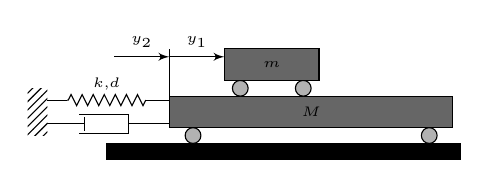
\begin{tikzpicture}[
        >=latex',
        spring/.style = {decorate,decoration={zigzag,amplitude=2pt,segment length=4pt}},
        damper/.style = {decorate,decoration={markings, mark connection node=dmp, mark=at position 0.5 with {
            \node (dmp) [thick,inner sep=0pt,transform shape,rotate=-90,minimum width=6pt,minimum height=15pt,draw=none] {};
            \draw ($(dmp.north east)+(2pt,0)$) -- (dmp.south east) -- (dmp.south west) -- ($(dmp.north west)+(2pt,0)$);
            \draw ($(dmp.north)+(0,-2.5pt)$) -- ($(dmp.north)+(0,2.5pt)$);
        }
        }}
    ]
    \draw[black, fill=black] (-0.5, 0) rectangle (4, 0.2);
    \draw[black, fill=black!30] (3.6,0.3) circle (0.1);
    \draw[black, fill=black!30] (0.6,0.3) circle (0.1);
    \draw[black, fill=black!60] (0.3, 0.4) rectangle (3.9, .8) node[pos=.5] {\tiny$M$};
    \draw[black, fill=black!30] (1.2, 0.9) circle (0.1);
    \draw[black, fill=black!30] (2,0.9) circle (0.1);
    \draw[black, fill=black!60] (1, 1) rectangle (2.2, 1.4) node[pos=.5] {\tiny$m$};
    \draw[black] (0.3,0.8) -- (0.3, 1.4);
    \draw[black] (0.3, 0.75) -- (0, 0.75);
    \draw[black] (0.3, 0.45) -- (0, 0.45);
    \draw[spring] (0,0.75) -- node[above] {\tiny$k$,$d$} +(-1,0);
    \draw[damper] (0,0.45) -- +(-1,0);
    \draw[black] (-1, 0.75) -- (-1.25, 0.75);
    \draw[black] (-1, 0.45) -- (-1.25, 0.45);
    \draw[fill,pattern=north east lines,draw=none,minimum width=0.75cm,minimum height=0.3cm,inner sep=0pt,outer sep=0pt] (-1.5, 0.3) rectangle
    (-1.25, 0.9);
    \draw[<-] (0.3, 1.3) -- node[above] {\tiny$y_2$} +(-0.7, 0);
    \draw[->] (0.3, 1.3) -- node[above] {\tiny$y_1$}(1,1.3);
\end{tikzpicture}

	%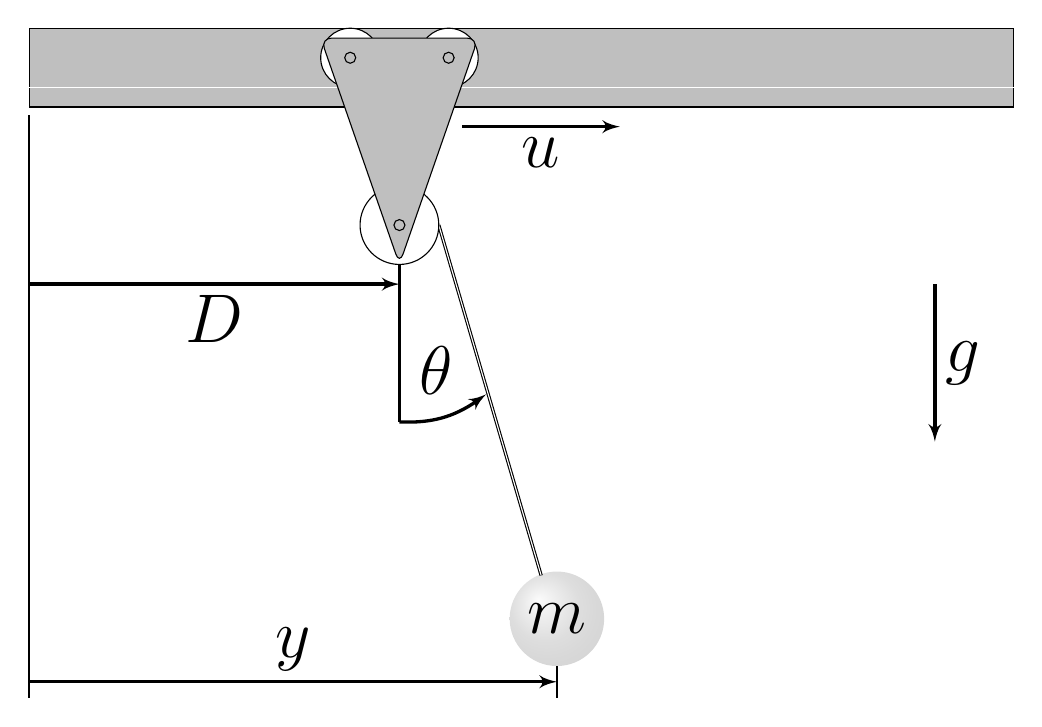
\begin{tikzpicture}[auto, >=latex']

    \draw[black, thick] (12.5, 2) -- (12.5, 9.4);
    \draw[black, thick] (19.2, 2.0) -- (19.2, 2.4);
    \draw[black, thick] (17.2, 5.5) -- (17.2, 7.5);

    \draw[fill=lightgray] (12.5,10.5) rectangle (25,9.5);

    \draw[color=white] (12.5,9.75) -- (25,9.75);
    % Kabel
    \draw[double distance=0.4] (17.7,8) -- ++(1.3,-4.45);
    \draw[fill=white] (17.2,8) circle (0.5);
    \draw[fill=white] (17.825,10.125) circle (0.375) +(-1.25,0) circle (0.375);
    \draw[rounded corners, fill=lightgray] (17.2,7.5) -- (18.2,10.375) -- ++(-2,0) -- cycle;
    \draw (17.2,8) circle (0.07);
    \draw (17.825,10.125) circle (0.07) +(-1.25,0) circle (0.07);
    % last
    \shade[ball color=black!50!white,opacity=0.20] (19.2, 3.) circle (0.6) node [opacity=1]{\Huge $m$};

    \draw[->, very thick] (17.2,5.5) to [bend right=20] node [above, xshift=-0.75ex,yshift=1ex] {\Huge $\theta$} (18.3,5.85);
    \draw[->, very thick] (12.5, 2.2) -- node [above] {\Huge $y$} (19.2, 2.2);
    \draw[->, very thick] (12.5, 7.25) -- node [below] {\Huge $D$} (17.2, 7.25);
    \draw[->, very thick] (18, 9.25) -- node [below] {\Huge $u$} (20, 9.25);
    \draw[->, very thick] (24, 7.25) -- node [right] {\Huge $g$} (24, 5.25);
\end{tikzpicture}

    %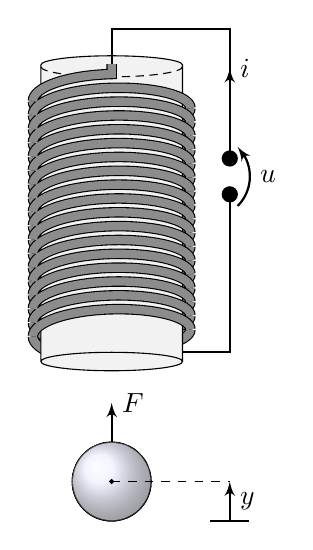
\begin{tikzpicture}[auto, >=latex']
	\draw[decoration={aspect=0.3,segment length=3mm,amplitude=10mm,coilup,segment length=5pt},decorate,double=gray!90,double distance=3pt] (0,1.5) -- (0,5.3);
	\node[cylinder,fill=gray!10,rotate=270,draw,minimum height=4.0cm,minimum width=1.8cm,anchor=east] at (0,1.4) (A) {};
	\draw[densely dashed] (-0.9,5.27) arc (180:0:0.9cm and -0.13cm);
	\draw[decoration={aspect=0.3,segment length=3mm,amplitude=10mm,coildown,segment length=5pt},decorate,double=gray!90,double distance=3pt] (0,1.5) -- (0,5.3);

	\draw (-0.5,0) arc (180:360:0.5 and 0.5);
    \draw[dashed] (-0.5,0) arc (180:0:0.5 and 0.5);
    \draw (0,0.5) arc (90:270:0.5 and 0.5);
    \draw[dashed] (0,0.5) arc (90:-90:0.5 and 0.5);
    \draw (0,0) circle (0.5cm);
    \shade[ball color=blue!10!white,opacity=0.60] (0,0) circle (0.5);
    \draw[fill=black] (0,0) circle (0.025);

	\draw[-*, thick] (0.9, 1.65) -- (1.5,1.65) -- (1.5, 3.75);
    \draw[*->, thick] (1.5, 4) -- (1.5, 5.25) node [right] {$i$};
    \draw[-, thick] (1.5, 4.5) -- (1.5, 5.75) -- (0,5.75) -- (0,5.3) ;
    \draw[->, thick] (1.6, 3.5) to [bend left=-45] node [right] {$u$} (1.6, 4.25);

    \draw[->, thick] (0, 0.5) -- (0, 1) node [right] {$F$};

    \draw[->, thick] (1.5, -0.5) -- node [right] {$y$} (1.5, 0);
    \draw[-, thick] (1.25,-0.5) -- (1.75, -0.5);
    \draw[dashed] (0, 0) -- (1.5, 0);

\end{tikzpicture}

    %\tikzset{
    Heat/.style={
         draw=none,
         inner color=red,
         outer color=yellow,
            postaction={
                decorate,
                rounded corners=2pt,
                decoration={
                    markings,
                    mark=between positions 6pt and 55pt step 9pt
                    with {
                        \draw[-Triangle,red,line width=0.5pt](0,0)
                            --++(0.1,0.1)
                            --++(-0.2,0.1)
                            --++(0.1,0.1)
                            --++(0,0.2);
                    }
                }
            }
    },
    Cool/.style={
         draw=none,
            postaction={
                decorate,
                rounded corners=2pt,
                decoration={
                    markings,
                    mark=between positions 6pt and 55pt step 9pt
                    with {
                        \draw[-Triangle,blue,line width=0.5pt](0,0)
                            --++(0.1,0.1)
                            --++(-0.2,0.1)
                            --++(0.1,0.1)
                            --++(0,0.2);
                    }
                }
            }
      },
    CoolHeat/.style={
         draw=none,
            postaction={
                decorate,
                rounded corners=2pt,
                decoration={
                    markings,
                    mark=between positions 6pt and 55pt step 9pt
                    with {
                        \draw[-Triangle,blue!50!red,line width=0.5pt](0,0)
                            --++(0.1,0.1)
                            --++(-0.2,0.1)
                            --++(0.1,0.1)
                            --++(0,0.2);
                    }
                }
            }
      },
    Fan/.style={
        circle,
        draw,
        minimum size=1cm,
        path picture={
            \draw [black] (path picture bounding box.130) --
                    (path picture bounding box.15);
            \draw [black] (path picture bounding box.230) --
                    (path picture bounding box.345);
        },
        node contents={}
    }
}

\begin{tikzpicture}[auto, >=latex', every info/.style={font=\tiny}]

    \draw [thick] (0, -0.1) -- (6, -0.1);
    \draw [thick] (0, 1.775) -- (6, 1.775);
    \draw (4, 0.8375) node [Fan, minimum size=1.85cm] ;

    \draw [Heat, rotate=-90] (-1.375, 2) -- ++(0,4pt) -- ++(30pt,0) -- ++(0,-4pt);
    \draw [Cool, rotate=-90] (-1.7, 0) -- ++(0,4pt) -- ++(50pt,0) -- ++(0,-4pt);
    \draw [CoolHeat, rotate=-90] (-1.7, 5.25) -- ++(0,4pt) -- ++(50pt,0) -- ++(0,-4pt);

    \draw[thick] (3.6, 0.01) -- (3.6, -0.4);
    \draw[thick] (4.4, 0.01) -- (4.4, -0.4);
    \draw[thick] (4.4, -0.5) circle (0.1);
    \draw[thick] (3.6, -0.5) circle (0.1);
    \draw (4.4, -0.5) node [right] {$+$};
    \draw (3.6, -0.5) node [left] {$-$};

    \draw[thick] (1.2, -0.4) -- (1.2, 0.9) -- (1.6, 0.9) -- (1.8, 1.2) -- (2, 1.4);
    \draw[thick] (1.5, -0.4) -- (1.5, 0.8) -- (1.6, 0.8) -- (1.8, 0.5) -- (2, 0.3);
    \draw[thick] (1.5, -0.5) circle (0.1);
    \draw[thick] (1.2, -0.5) circle (0.1);
    \draw (1.5, -0.5) node [right] {$+$};
    \draw (1.2, -0.5) node [left] {$-$};
\end{tikzpicture}

\end{document}
